\def\mySecNum{10.1}
\mySection{\mySecNum~A one-period Binomial tree}
%-------------- start slide -------------------------------%{{{ 1
\begin{frame}[fragile,t]
	\frametitle{Binomial option pricing}
	\begin{center}

		The                                                        \\
		\textcolor{magenta}{\bf binomial option pricing model}     \\
		or                                                         \\
		\textcolor{magenta}{\bf Cox-Ross-Rubinstein pricing model} \\
		assumes that
		\bigskip

		the price of the underlying asset follows a binomial distribution,

		\bigskip
		that is,                                                   \\
		\bigskip


		the asset price in each period can                         \\
		move only up or down by a specified amount.

		\bigskip
		\mySeparateLine
		\bigskip

		The binomial option pricing model enables us to

		\begin{center}
			\textcolor{cyan}{determine the price of an option},
		\end{center}

		given the characteristics of the stock or other underlying asset.

	\end{center}
\end{frame}
%-------------- end slide -------------------------------%}}}
%-------------- start slide -------------------------------%{{{ 1
\begin{frame}[fragile,t]
\begin{myexample}
	\label{Eg:10-1}
	Consider an European call option on the stock of XYZ, with a \$40 strike price and one year
	expiration. XYZ does not pay dividends and its current price is \$41.
	\bigskip

	Assume that, in a year, the price can be either \$60 or \$30.
	\bigskip

	\begin{center}
		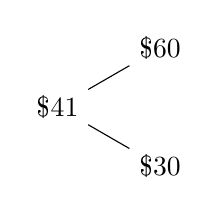
\begin{tikzpicture}[level distance=1.5cm,
			level 1/.style={sibling distance=3cm},
			level 2/.style={sibling distance=1.5cm}]
			\node {\$41}
				child[grow=30] {node {\$60}}
				child[grow=-30] {node {\$30}};
		\end{tikzpicture}
	\end{center}

	Can one determine the call premium?
	\bigskip

	(Let the continuously compounded risk free interest rate be 8\%.)
\end{myexample}
\end{frame}
%-------------- end slide -------------------------------%}}}
%-------------- start slide -------------------------------%{{{ 1
\begin{frame}[fragile,t]
\begin{center}
	\textcolor{magenta}{\it Law of one price}\\

	\bigskip
	Positions that have the same payoff should have the same cost!
	\bigskip
	\mySeparateLine
	\bigskip

	Two portfolios (positions)
	\bigskip

	\begin{itemize}
		\item Portfolio A: Buy one $40$-strike call option.
		\item Portfolio B: Buy $\Delta\in (0,1)$ share of stock and borrow $B$ at the risk-free rate.
	\end{itemize}
	\bigskip

	These two positions should have the same cost.
\end{center}
\end{frame}
%-------------- end slide -------------------------------%}}}
%-------------- start slide -------------------------------%{{{ 1
\begin{frame}[fragile,t]
\begin{mysol}
	The cost for Portfolio B at day zero is
	\begin{align*}
		\Delta \times S_0 - B.
	\end{align*}
	and its payoff at expiration is
	\begin{align*}
		\begin{cases}
			\Delta \times 30 - B\times e^{0.08} & \text{if the stock price is $30$} \\
			\Delta \times 60 - B\times e^{0.08} & \text{if the stock price is $60$}
		\end{cases}
	\end{align*}
	\bigskip

	On the other hand, the payoff for Portfolio A should be
	\begin{align*}
		\begin{cases}
			0       & \text{if the stock price is $30$} \\
			(60-40) & \text{if the stock price is $60$}
		\end{cases}
	\end{align*}

	\vfill
	By equating the two payoffs, one obtains that
	\begin{align*}
		\begin{cases}
			\Delta \times 30 - B\times e^{0.08} = 0 \\
			\Delta \times 60 - B\times e^{0.08} = 60-40
		\end{cases}
	\end{align*}
\end{mysol}
\end{frame}
%-------------- end slide -------------------------------%}}}
%-------------- start slide -------------------------------%{{{ 1
\begin{frame}[fragile,t]
\begin{mysol}
	Hence,
	\begin{align*}
		B = 20 \times e^{-0.08} \quad \text{and} \quad
		\Delta = 2/3.
	\end{align*}
	\bigskip

	Finally, since the cost of Portfolio A has to be equal to that of Portfolio B, we find the cost of Portfolio A:

	\begin{align*}
		\Delta \times S_0 - B = \frac{2}{3} S_0 - 20 \times e^{-0.08}.
	\end{align*}
	\bigskip

	If we plug in $S_0=\$41$, we have
	\begin{align*}
		B=\$18.462 \quad \text{and the cost is \$ 8.871.}
	\end{align*}
	\myEnd
\end{mysol}
\end{frame}
%-------------- end slide -------------------------------%}}}
%-------------- start slide -------------------------------%{{{ 1
\begin{frame}[fragile,t]
More generally, suppose the stock change its value over a period of time $h$ as
\begin{center}
	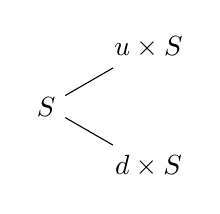
\begin{tikzpicture}[level distance=1.5cm,
		level 1/.style={sibling distance=3cm},
		level 2/.style={sibling distance=1.5cm}]
		\node {$S$}
			child[grow=30] {node {$u\times S$}}
			child[grow=-30] {node {$d \times S$}};
	\end{tikzpicture}
	\mySeparateLine
	\bigskip

	Portfolio A
	\bigskip

	\renewcommand{\arraystretch}{1.2}
	\begin{tabular}{|c|c|c|}
		\hline
    Payoff & $d \times S$              & $u\times S$                             \\ \hline
    Option & $0$                       & $u\times S-K$                           \\ \hline \hline
		Total  & $\textcolor{cyan}{C_d=0}$ & $\textcolor{magenta}{C_u= u\cdot S -K}$ \\
	 \hline
	\end{tabular}

	\bigskip

	Portfolio B
	\bigskip

	\renewcommand{\arraystretch}{1.2}
	\begin{tabular}{|c|c|c|}
		\hline
    Payoff         & $d \times S$                                                          & $u\times S$                                                                 \\ \hline
		$\Delta$ share & $\Delta\cdot d\cdot S\cdot e^{\delta h}$                              & $\Delta \cdot u \cdot S \cdot e^{\delta h}$                                 \\
		$B$ bond       & $B e^{rh}$                                                            & $ B e^{rh}$                                                                 \\ \hline \hline
		Total          & $\textcolor{cyan}{\Delta\cdot d\cdot S\cdot e^{\delta h} + B e^{rh}}$ & $\textcolor{magenta}{\Delta \cdot u \cdot S \cdot e^{\delta h} + B e^{rh}}$ \\ \hline
	\end{tabular}
\end{center}
\end{frame}
%-------------- end slide -------------------------------%}}}
%-------------- start slide -------------------------------%{{{ 1
\begin{frame}[fragile,t]
	\begin{center}
		For two unknowns: $\Delta$ and  $B$, solve:
	\end{center}
	\begin{align*}
		\begin{cases}
			\displaystyle \textcolor{cyan}{\Delta d S e^{\delta h} + B e^{rh} = C_d}    \\[1em]
			\displaystyle \textcolor{magenta}{\Delta u S e^{\delta h} + B e^{rh} = C_u} \\
		\end{cases}
	\end{align*}

	\bigskip
	\mySeparateLine
	\bigskip
	\begin{center}
		Set $S_h$	be either $dS$ or  $uS$ and \\
		$C_h$	be either $C_u$ or  $C_d$. \\
		Plot \textcolor{magenta}{$S_h$ ($x$-axis)} versus  \textcolor{cyan}{$C_h$ ($y$-axis)}.
	\end{center}
	\begin{align*}
		\Delta \textcolor{magenta}{S_h} e^{\delta h} + B e^{rh} =\textcolor{cyan}{C_h}
	\end{align*}
\end{frame}
%-------------- end slide -------------------------------%}}}
%-------------- start slide -------------------------------%{{{ 1
\begin{frame}[fragile,t]
\begin{center}
	\includegraphics[scale=0.25]{figs/Figure-10-2.png}
\end{center}
\end{frame}
%-------------- end slide -------------------------------%}}}
%-------------- start slide -------------------------------%{{{ 1
\begin{frame}[fragile,t]
\begin{align*}
	\Delta = e^{-\delta h}	\frac{C_h-C_d}{S(u-d)} \qquad \text{and} \qquad
	B = e^{-r h}	\frac{uC_d-dC_u}{u-d}
\end{align*}
\bigskip
\begin{align*}
	\Delta S + B = e^{-rh}\bigg(C_u \underbrace{\frac{e^{(r-\delta)h}-d}{u-d}}_{:=p^*} + C_d \underbrace{\frac{u-e^{(r-\delta) h}}{u-d}}_{:=1-p^*}\bigg)
\end{align*}
\bigskip
\begin{center}
	$p^*$ the \textcolor{magenta}{\bf risk-neutral probability} of \\
	an increase in the stock price.
\end{center}
\end{frame}
%-------------- end slide -------------------------------%}}}
%-------------- start slide -------------------------------%{{{ 1
\begin{frame}[fragile,t]
	\frametitle{Arbitraging a mispriced option}
	\begin{myexample}
		Find arbitrage opportunities in Example \myref{Eg:10-1} with
		\begin{itemize}
			\item the option price being overpriced with \$9.00;
			\item the option price being underpriced with \$8.25,
		\end{itemize}
		\pause
		instead of the risk-neutral pricing \$8.871.
	\end{myexample}
	\bigskip
	\pause
	\begin{mysol}
		One can buy the synthetic option which cost \$8.25 and sell the real one by earning \$9.00.
		Hence, the present value of the profit is
		\begin{align*}
			\$ 9 - \$ 8.871 = \$ 0.129.
		\end{align*}
		\myEnd
	\end{mysol}
\end{frame}
%-------------- end slide -------------------------------%}}}
